\section{Phần dịch trang 0 đến 10}
Chương 5 Logic chương trình và Vòng lặp vô định (Indefinite Loops)

\subsection*{5.1 Vòng lặp while}
\begin{itemize}
    \item Vòng lặp tìm ước số nhỏ nhất
    \item Số ngẫu nhiên (Random Numbers)
    \item Mô phỏng (Simulations)
    \item Vòng lặp do/while
\end{itemize}

\subsection*{5.2 Thuật toán Fencepost}
\begin{itemize}
    \item Fencepost với if
    \item Vòng lặp Sentinel (Sentinel Loops)
\end{itemize}

\subsection*{5.3 Kiểu dữ liệu boolean}
\begin{itemize}
    \item Các toán tử logic (Logical Operators)
    \item Đánh giá ngắn mạch (Short-Circuited Evaluation)
    \item Biến boolean và Cờ hiệu (Flags)
    \item Thiền Boolean (Boolean Zen)
    \item Phủ định biểu thức Boolean
\end{itemize}

\subsection*{5.4 Lỗi người dùng}
\begin{itemize}
    \item Kỹ thuật Scanner Lookahead
    \item Xử lý lỗi người dùng
\end{itemize}

\subsection*{5.5 Khẳng định (Assertions) và Logic chương trình}
\begin{itemize}
    \item Lập luận về các Khẳng định
    \item Ví dụ chi tiết về Khẳng định
\end{itemize}

\subsection*{5.6 Nghiên cứu điển hình: NumberGuess}
\begin{itemize}
    \item Phiên bản đầu tiên không có gợi ý
    \item Phiên bản ngẫu nhiên có gợi ý
    \item Phiên bản hoàn chỉnh chống lỗi (Robust Version)
\end{itemize}

\subsection*{Giới thiệu}
Chương này bắt đầu bằng việc nghiên cứu một cấu trúc mới gọi là vòng lặp \texttt{while}, cho phép bạn lặp lại một số lần vô định (indefinite number of times). Vòng lặp \texttt{while} sẽ cho phép bạn giải quyết một lớp bài toán lập trình mới mà trong đó bạn không biết trước mình muốn vòng lặp thực thi bao nhiêu lần. Ví dụ, các chương trình chơi game thường liên quan đến vòng lặp \texttt{while} vì không thể biết trước người dùng sẽ chơi game như thế nào. Bởi vì chúng ta sẽ khám phá các chương trình trò chơi, chúng ta cũng sẽ tìm hiểu cách tạo số ngẫu nhiên bên trong một chương trình Java. Chúng ta cũng sẽ khám phá một lớp thuật toán khác được gọi là thuật toán fencepost (thuật toán hàng rào) thường xuất hiện trong các tác vụ lập trình vòng lặp.

Sau đó, chương này sẽ thảo luận về kiểu dữ liệu nguyên thủy thứ tư mà chúng ta sẽ nghiên cứu chi tiết, \texttt{boolean}. Kiểu \texttt{boolean} được sử dụng để lưu trữ thông tin logic (đúng/sai - true/false). Khi bạn đã hiểu chi tiết về kiểu \texttt{boolean}, bạn sẽ có thể viết các vòng lặp phức tạp liên quan đến nhiều điều kiện kiểm tra.

Tiếp theo, chúng ta sẽ xem xét ngắn gọn chủ đề quan trọng về xử lý lỗi của người dùng.

Chương này kết thúc bằng cuộc thảo luận về các khẳng định (assertions). Bằng cách sử dụng các khẳng định, bạn có thể lập luận về các thuộc tính hình thức của chương trình (điều gì là đúng tại các thời điểm khác nhau trong quá trình thực thi chương trình).

\subsection*{5.1 Vòng lặp while}
Các vòng lặp \texttt{for} mà chúng ta đã viết từ Chương 2 là các vòng lặp khá đơn giản, thực thi một số lần có thể dự đoán được. Hãy nhớ rằng chúng ta gọi chúng là vòng lặp xác định (definite loops) vì chúng ta biết chính xác chúng sẽ thực thi bao nhiêu lần trước khi vòng lặp bắt đầu chạy. Bây giờ chúng ta muốn chuyển sự chú ý sang các vòng lặp vô định (indefinite loops), thực thi một số lần chưa biết trước. Vòng lặp vô định thường xuất hiện trong các chương trình tương tác và xử lý tệp. Ví dụ, bạn không biết trước một người dùng muốn chơi một trò chơi bao nhiêu lần, và bạn sẽ không biết trước khi xem một tệp chính xác lượng dữ liệu mà nó lưu trữ.

Vòng lặp \texttt{while} là vòng lặp vô định đầu tiên chúng ta sẽ nghiên cứu. Nó có cú pháp như sau:

\begin{verbatim}
while (<test>) {
    <statement>;
    <statement>;
     ...
    <statement>;
}
\end{verbatim}

Sơ đồ trong Hình 5.1 chỉ ra luồng điều khiển của vòng lặp \texttt{while}. Vòng lặp thực hiện kiểm tra điều kiện của nó và nếu điều kiện đánh giá là \texttt{true}, nó sẽ thực thi các câu lệnh được kiểm soát. Nó liên tục kiểm tra và thực thi nếu điều kiện đánh giá là \texttt{true}. Chỉ khi điều kiện đánh giá là \texttt{false} thì vòng lặp mới kết thúc.

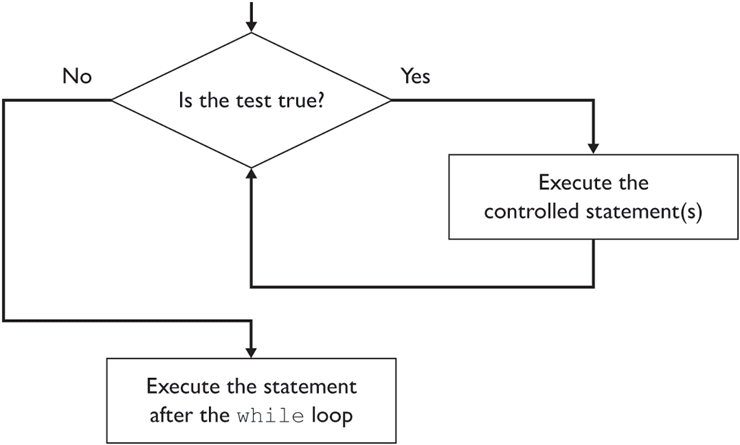
\includegraphics{Pictures/ch05_p4_img0.png}
\\
\textit{Hình 5.1: Luồng hoạt động của vòng lặp while}

Như Hình 5.1 chỉ ra, vòng lặp \texttt{while} thực hiện kiểm tra điều kiện ở phần đầu của vòng lặp, trước khi thân vòng lặp được thực thi. Một vòng lặp \texttt{while} sẽ không thực thi các câu lệnh được kiểm soát của nó nếu điều kiện của nó đánh giá là \texttt{false} ngay trong lần đầu tiên nó được đánh giá.

Dưới đây là một ví dụ về vòng lặp \texttt{while}:

\begin{verbatim}
int number = 1;
while (number <= 200) {
    number = number * 2;
}
\end{verbatim}

Vòng lặp này khởi tạo một biến số nguyên tên là \texttt{number} bằng 1 và sau đó nhân đôi nó trong khi nó nhỏ hơn hoặc bằng 200. Nhìn bề ngoài, hoạt động này tương tự như việc sử dụng câu lệnh \texttt{if}:

\begin{verbatim}
int number = 1;
if (number <= 200) {
    number = number * 2;
}
\end{verbatim}

Sự khác biệt giữa hai dạng này là vòng lặp \texttt{while} thực thi nhiều lần, lặp lại cho đến khi điều kiện kiểm tra đánh giá là \texttt{false}. Câu lệnh \texttt{if} chỉ thực thi câu lệnh nhân đôi một lần duy nhất, để lại \texttt{number} bằng 2. Vòng lặp \texttt{while} thực thi câu lệnh nhân đôi lặp đi lặp lại, với \texttt{number} nhận các giá trị 1, 2, 4, 8, 16, 32, 64, 128, và 256. Vòng lặp không dừng thực thi cho đến khi điều kiện kiểm tra đánh giá là \texttt{false}. Nó thực thi câu lệnh gán tám lần và kết thúc khi \texttt{number} được đặt thành giá trị 256 (lũy thừa đầu tiên của 2 lớn hơn 200).

Dưới đây là một vòng lặp \texttt{while} chứa hai câu lệnh:

\begin{verbatim}
int number = 1;
while (number <= max) {
    System.out.println("Hi there");
    number++;
}
\end{verbatim}

Vòng lặp \texttt{while} này gần như giống hệt với vòng lặp \texttt{for} sau:

\begin{verbatim}
for (int number = 1; number <= max; number++) {
    System.out.println("Hi there");
}
\end{verbatim}

Sự khác biệt duy nhất giữa hai vòng lặp này là phạm vi hoạt động (scope) của biến \texttt{number}. Trong vòng lặp \texttt{while}, \texttt{number} được khai báo trong phạm vi bên ngoài vòng lặp. Trong vòng lặp \texttt{for}, \texttt{number} được khai báo bên trong vòng lặp.

\subsection*{Vòng lặp tìm ước số nhỏ nhất}
Giả sử bạn muốn tìm ước số nhỏ nhất của một số khác 1. Bảng 5.1 đưa ra các ví dụ về những gì bạn đang tìm kiếm.

\textit{Bảng 5.1: Ví dụ về các ước số}

Dưới đây là mô tả bằng mã giả (pseudocode) về cách bạn có thể tìm giá trị này:

\begin{verbatim}
bắt đầu divisor tại 2.
while (giá trị hiện tại của divisor không chia hết) {
    tăng divisor.
}
\end{verbatim}

Bạn không bắt đầu \texttt{divisor} tại 1 vì bạn đang tìm kiếm ước số đầu tiên lớn hơn 1. Để tinh chỉnh mã giả này, bạn phải rõ ràng hơn về điều gì làm cho một ước số "chia hết". Một ước số của một số sẽ không có số dư khi số đó được chia cho ước số đó. Bạn có thể viết lại quy tắc này dưới dạng mã giả sau:

\begin{verbatim}
bắt đầu divisor tại 2.
while (số dư của number/divisor không bằng 0) {
    tăng divisor.
}
\end{verbatim}

Bài toán này có thể được giải quyết bằng cách sử dụng toán tử chia lấy dư \texttt{\%}, toán tử này cho biết số dư của phép chia số nguyên. Vòng lặp \texttt{while} sau đây thực hiện tác vụ đó:

\begin{verbatim}
int divisor = 2;
while (number % divisor != 0) {
    divisor++;
}
\end{verbatim}

Một vấn đề mà bạn chắc chắn sẽ gặp phải khi viết vòng lặp \texttt{while} là vòng lặp vô hạn (infinite loop) khét tiếng. Hãy xem xét đoạn mã sau:

\begin{verbatim}
int number = 1;
while (number > 0) {
    number++;
}
\end{verbatim}

Bởi vì \texttt{number} bắt đầu là một giá trị dương và vòng lặp làm cho nó lớn hơn, vòng lặp này sẽ tiếp tục vô tận. Bạn phải cẩn thận khi xây dựng các vòng lặp \texttt{while} của mình để tránh các tình huống mà một đoạn mã sẽ không bao giờ kết thúc quá trình thực thi. Mỗi khi bạn viết một vòng lặp \texttt{while}, bạn nên cân nhắc xem khi nào và làm thế nào nó sẽ kết thúc thực thi.

\subsection*{LỖI LẬP TRÌNH PHỔ BIẾN: Vòng lặp vô hạn}
Viết một vòng lặp \texttt{while} không bao giờ kết thúc là điều tương đối dễ mắc phải. Một lý do khiến lỗi này dễ xảy ra là vòng lặp \texttt{while} không có bước cập nhật trong phần đầu của nó như vòng lặp \texttt{for}. Điều quan trọng là lập trình viên phải đưa vào một bước cập nhật chính xác vì bước này là cần thiết để cuối cùng làm cho điều kiện kiểm tra của vòng lặp bị thất bại (trả về \texttt{false}).

Hãy xem xét đoạn mã sau, được thiết kế để yêu cầu người dùng nhập một số và liên tục in ra số đó được giảm đi một nửa cho đến khi đạt đến 0. Lần thử đầu tiên này không biên dịch được:

\begin{verbatim}
Scanner console = new Scanner(System.in);
System.out.print("Type a number: "); 
 
// đoạn mã này không biên dịch được
while (number > 0) {
    int number = console.nextInt();
}
\end{verbatim}